\section{theorem14(intergenerator theorem)}
\begin{theorem}
\end{theorem}

Suppose we have an intergenerator diagram on $n$ strands and an intergenerator sheaf on it. If we apply intergenerator move to the diagram, then we get the following diagram and a sheaf :

\begin{figure}[H] % Optional: [h] means here, [t] for top, [b] for bottom, [p] for page of floats
    \centering
    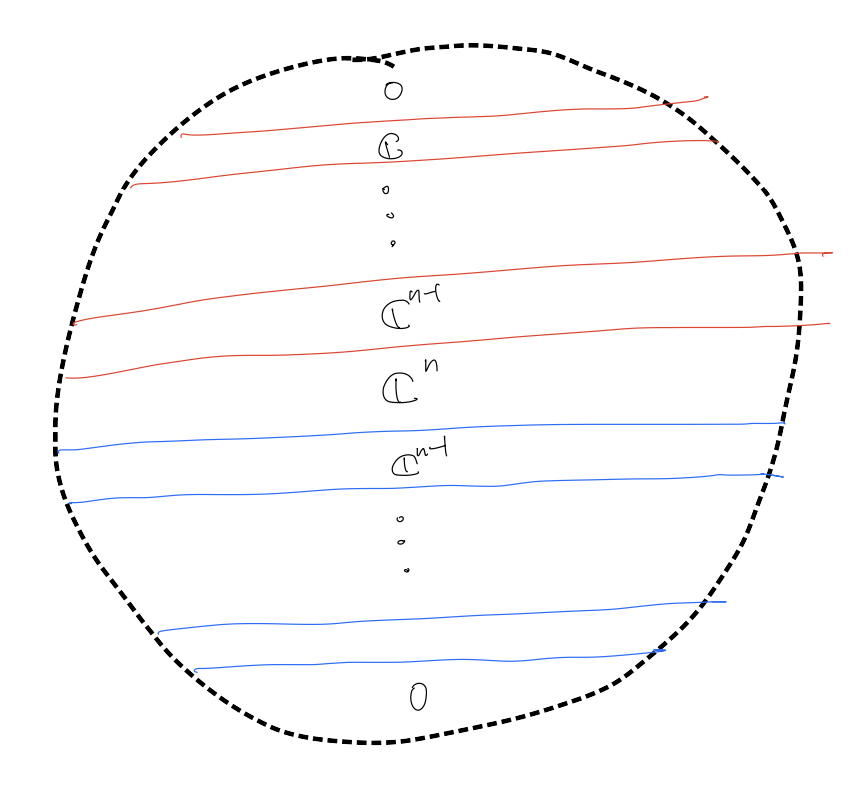
\includegraphics[width=\linewidth]{diagrams/theorem14/1.png} % Adjust the width as needed
    \caption{Your caption here}
    \label{fig:your-label}
\end{figure}

(proof) We prove the statement by induction. If $n=1$, then the intergenerator move is the null move. So the statement holds trivially. If $n>1$, then by induction hypothesis, after applying intergenerator move to intergenerator diagram on $n-1$ strands inside the middle circle

\begin{figure}[H] % Optional: [h] means here, [t] for top, [b] for bottom, [p] for page of floats
    \centering
    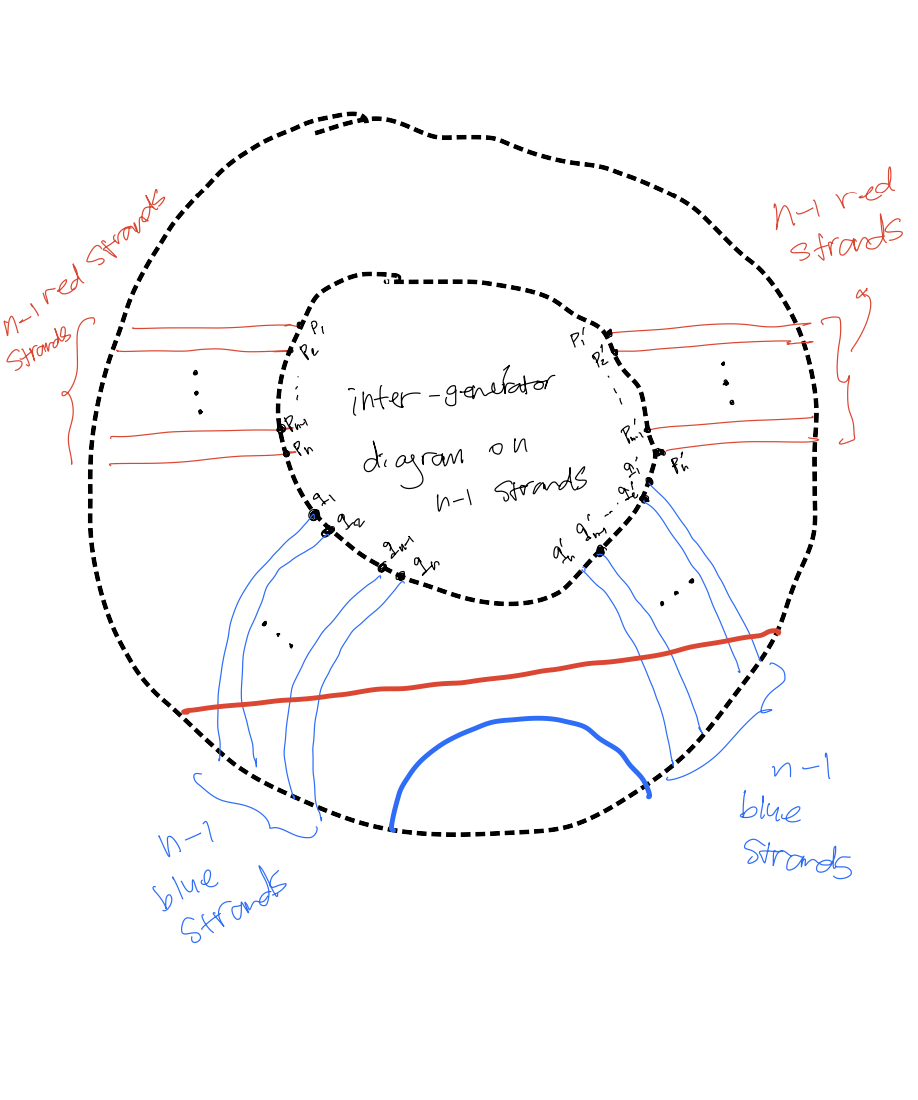
\includegraphics[width=\linewidth]{diagrams/theorem14/2.png} % Adjust the width as needed
    \caption{Your caption here}
    \label{fig:your-label}
\end{figure}

we get :

\begin{figure}[H] % Optional: [h] means here, [t] for top, [b] for bottom, [p] for page of floats
    \centering
    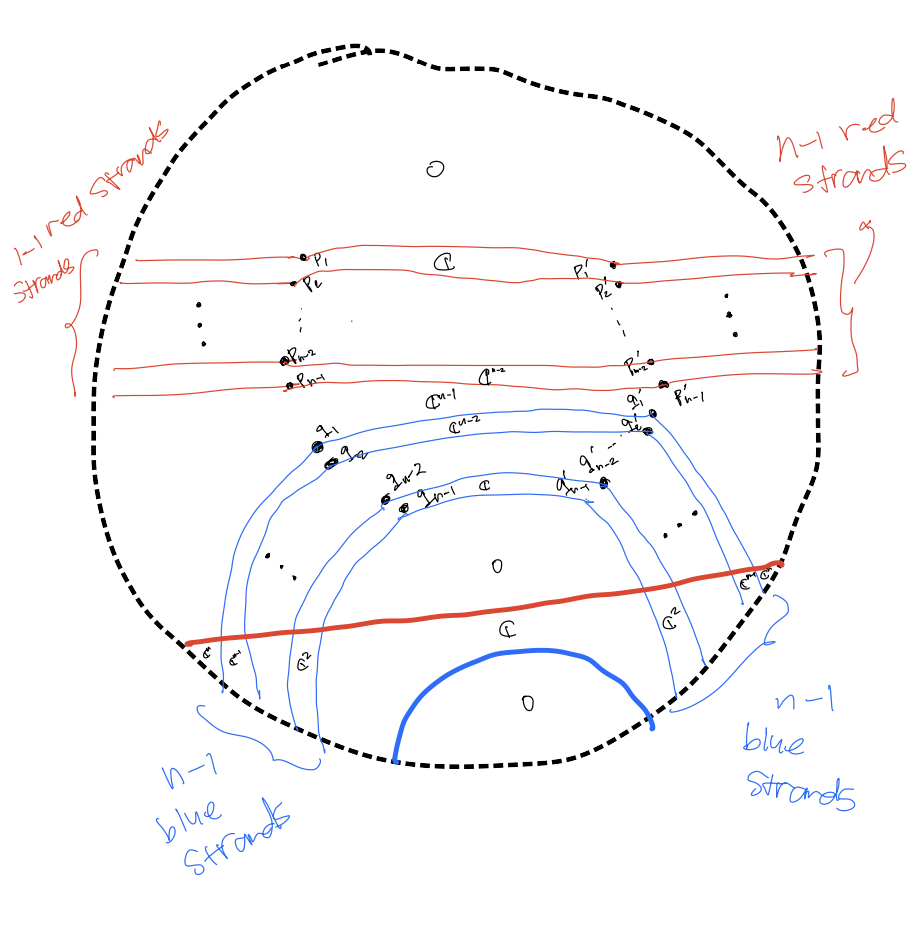
\includegraphics[width=\linewidth]{diagrams/theorem14/3.png} % Adjust the width as needed
    \caption{Your caption here}
    \label{fig:your-label}
\end{figure}

After applying MOVE \RN{13}, by Theorem 13, we get

\begin{figure}[H] % Optional: [h] means here, [t] for top, [b] for bottom, [p] for page of floats
    \centering
    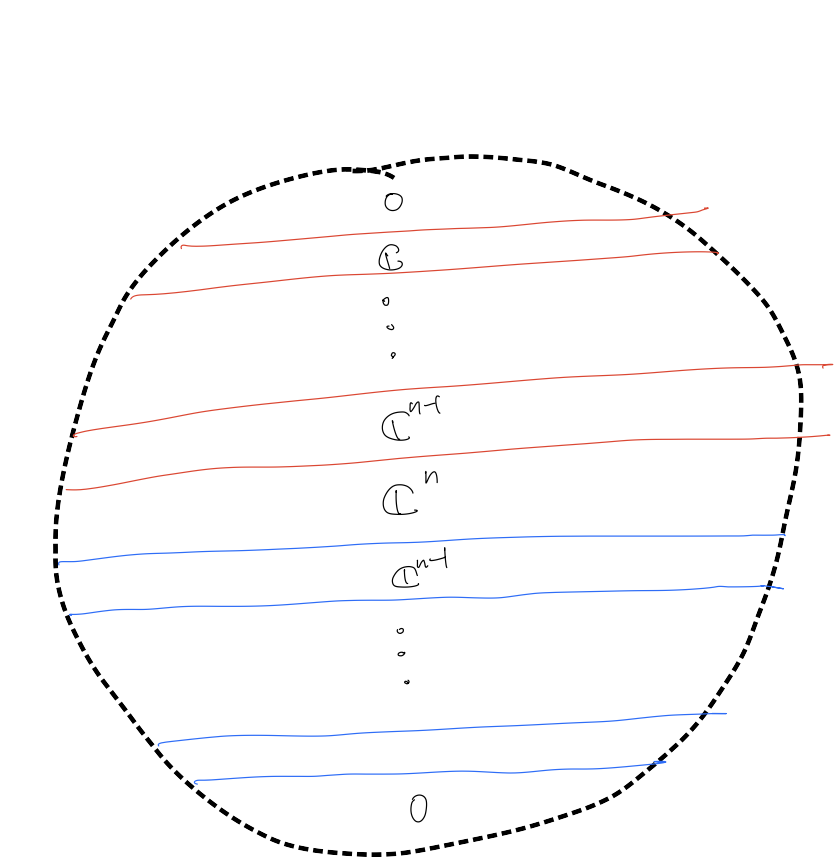
\includegraphics[width=\linewidth]{diagrams/theorem14/4.png} % Adjust the width as needed
    \caption{Your caption here}
    \label{fig:your-label}
\end{figure}